\section{aTag Enhancements}
We have demonstrated a tag format consisting of an attribute superset identifier and an bitmask, which can be used for easily decoding attributes associated with a flow. We will now present some improvements to this format.

%\subsection{Encoding Non-Binary Attributes}


\subsection{Variable Length Identifiers}
It is unlikely that all attribute supersets will be the same width, causing different tags to use a different number of bits. If we are using a fixed-width field in the packet headers for the tags, then it must be at least the size of the largest tag, and all smaller tags must be padded to the size of the largest tag. This wastes space which could perhaps be used in a more clever fashion.

\begin{figure}[t!] 
\begin{minipage}{1\linewidth}
\begin{subfigure}[c]{0.96\linewidth}
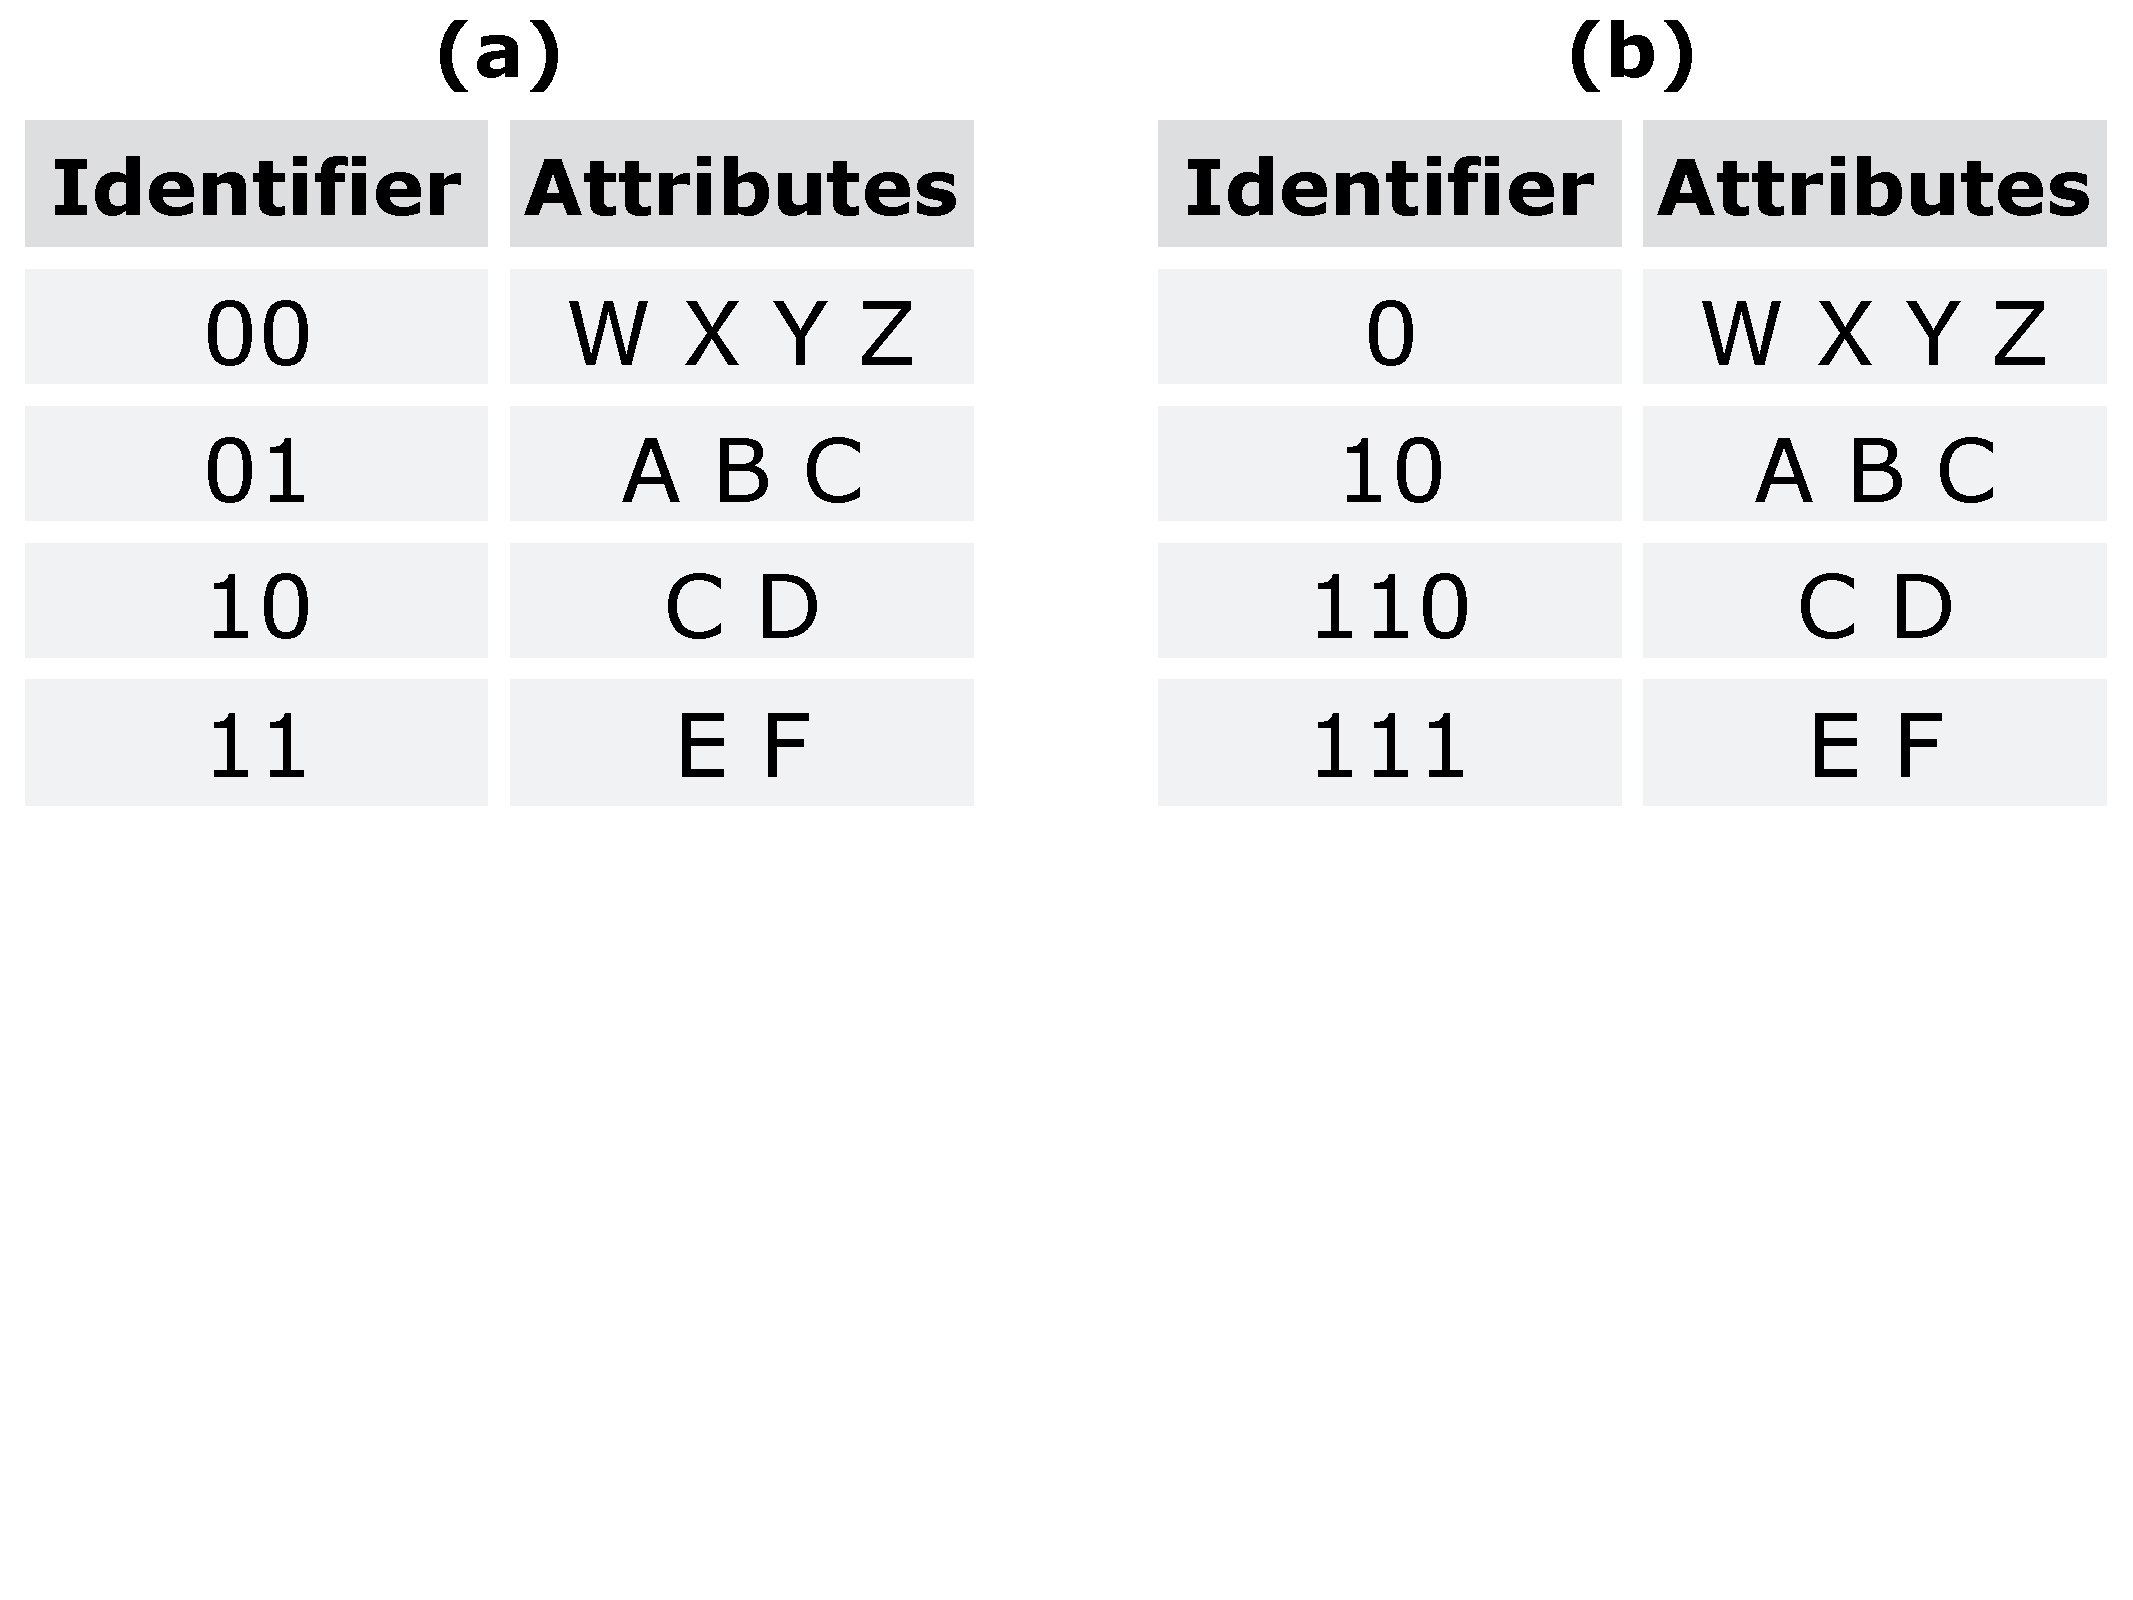
\includegraphics[trim={0 7cm 18cm 0}, clip, width=\linewidth]{figures/variable_identifiers}
\end{subfigure} 
\end{minipage} 
\caption{(a) shows example supersets with fixed-length identifiers. (b) shows variable-length identifiers for the same supersets. With variable length identifiers, the maximum tag width is reduced from 6 to 5 bits. (c) shows how variable-length identifiers can be built from the leaves of a binary tree.}
\label{fig:variable_id}
\end{figure}

Figure \ref{fig:variable_id}(a) shows an example list of supersets, where the tag width is determined by one large superset. If the largest superset had a smaller identifier than the other supersets, the tag width could be decreased. However, if each tag has a different length identifier, then it unclear where the boundary between the identifier and the mask lies in any given tag. We can circumvent this with the use of prefix codes. A prefix code is a set of codewords such that no codeword is a prefix of any other codeword. Figure \ref{fig:variable_id}(b) shows an example prefix code identifier assignment, which decreases the overall tag width from 6 bits to 5 bits. Figure \ref{fig:variable_id}(c) shows how these codewords can be built from the leaves of a binary tree. To read a codeword from left to right, you begin at the root of the tree and go to the left child if you read a $0$ and right if you read a $1$. Once a leaf node is reached, the identifier has been fully read.

\subsection{Width with Variable Length Identifiers}
We discussed the used of prefix codes to take advantage of the variable amount of space available for superset identifiers. We can determine the optimal width possible from using a prefix free code with Kraft's Inequality. Kraft's inequality states that, given a requirement of $N$ codewords where each codeword has a limited width of $L_i$, then it is possible to construct a prefix code if the following equation is satisfied:
$$ \sum_{i = 0}^{N}{2^{-L_i} \le 1} $$
Where, in our case, $L_i$ is the maximum width available for the $i^{th}$ superset's identifying codeword. We can use this inequality to determine the smallest tag width possible, denoted by $W_{min}$, for a given list of supersets. Note that, for the $i^{th}$ superset, the space available for the identifying codeword will be $L_i = W_{min} - |superset_i|$. Using this, we can solve for $W_{min}$.\\

\begin{equation} \label{eq1}
 \begin{split}
  \sum_{i = 0}^{N}{2^{-(W_{min} - |superset_i|)}}   \le  1 \\
  \implies 2^{-W_{min}} \sum_{i = 0}^{N}{2^{|superset_i|}}   \le  1 \\
  \implies  \sum_{i = 0}^{N}{2^{|superset_i|}}   \le  2^{W_{min}} \\
 \implies   \lceil\log_2{\sum_{i = 0}^{N}{2^{|superset_i|}}}\rceil  =  W_{min}
\end{split}
 \end{equation}
 
 The left hand side is straightforward to solve, giving us the minimum width possible for the input list of supersets. We can then use this value to find each $L_i$, or the width available for the identifier of the $i^{th}$ superset.
 
 Once all the identifier widths are known, finding an actual prefix code can be accomplished by building a binary code tree. Figure \ref{fig:variable_id}(c) shows such a code tree. Each node $n$ in the tree is associated with a binary string $s$. The left child of $n$ will have string $s + '0'$, and the right child will have $s + '1'$. The root of the tree corresponds to the empty string. A consequence of this is that node in the tree is a prefix of all of its children. To construct a prefix code, only leaf nodes may be codewords. 
 
 The code is built with a level-by-level tree construction. We begin with level 0, the root node. Two children are added to the root to create level 1, corresponding to strings $'0'$ and $'1'$, the length 1 binary strings. The construction proceeds as follows:  After creating the $k^th$ level of the tree, if there exists an $i$ such that $L_i = k$, we assign an arbitrary node in the current level to be the $i^th$ codeword. After all such codewords are assigned, the next level is constructed. Child node are added for each node in the current level that was not assigned as a codeword, and the construction proceeds until all codewords are assigned.
 
\subsubsection{Minimizing Kraft to Decrease Tag Width}
We've shown how to find a prefix code which optimally minimizes the tag width for a fixed list of supersets, but the problem becomes more interesting if we are permitted to modify the list of supersets. 

Recall that the tag width $W_min$ for a list of supersets is given by the equation $W_{min} = \lceil\log_2{\sum_{i = 0}^{N}{2^{|superset_i|}}}\rceil$. If we can reduce the sum within the log term, we may be able to decrease the width. This can be done with a simple greedy algorithm. Consider every pair of supersets. Find the pair which, when removed and replaced by their union, maximally decreases the sum ${\sum_{i = 0}^{N}{2^{|superset_i|}}}$. If no union decreases the sum, instead choose the union that minimally increases it. If this union operation increases $W_min$, stop. Otherwise, perform the union and then repeat. 

